% !TEX root = ../tjumain.tex
\chapter{任务要求}

\section{可靠数据传输}

\begin{enumerate}
  \item 需要在两端设置、管理发送和接收缓冲区,实现滑动窗口的机制(我们采用了 AVL,自平衡二叉搜索树的数据结构提升效率)
  \item 需要依照 RFC793 Sec 3.7 的描述实现并行的可靠数据传输(即流水线技术)
  \item 需要依照 RFC793 Sec 3.7 的描述估计 RTT,计算 RTO,并根据 RTO 进行数据包的超时重传
  \item 能够在有不可靠的链路上实现至少 100 MB 数据的传输
\end{enumerate}

\section{流量控制}
\begin{enumerate}
  \item 发送方根据 “advertised window" 字段的信息调整发送窗口
  \item 依据 RFC 793 Sec 3.7 的标准实现发送方应对接收方0窗口情况并进行规避
\end{enumerate}

\section{环境和语言}

使用指定的Linux操作系统,C语言实现TJU\_TCP协议。 系统配置如图\ref{fig:ubuntu} 所示。

\begin{figure}[!htbp]
    \centering
    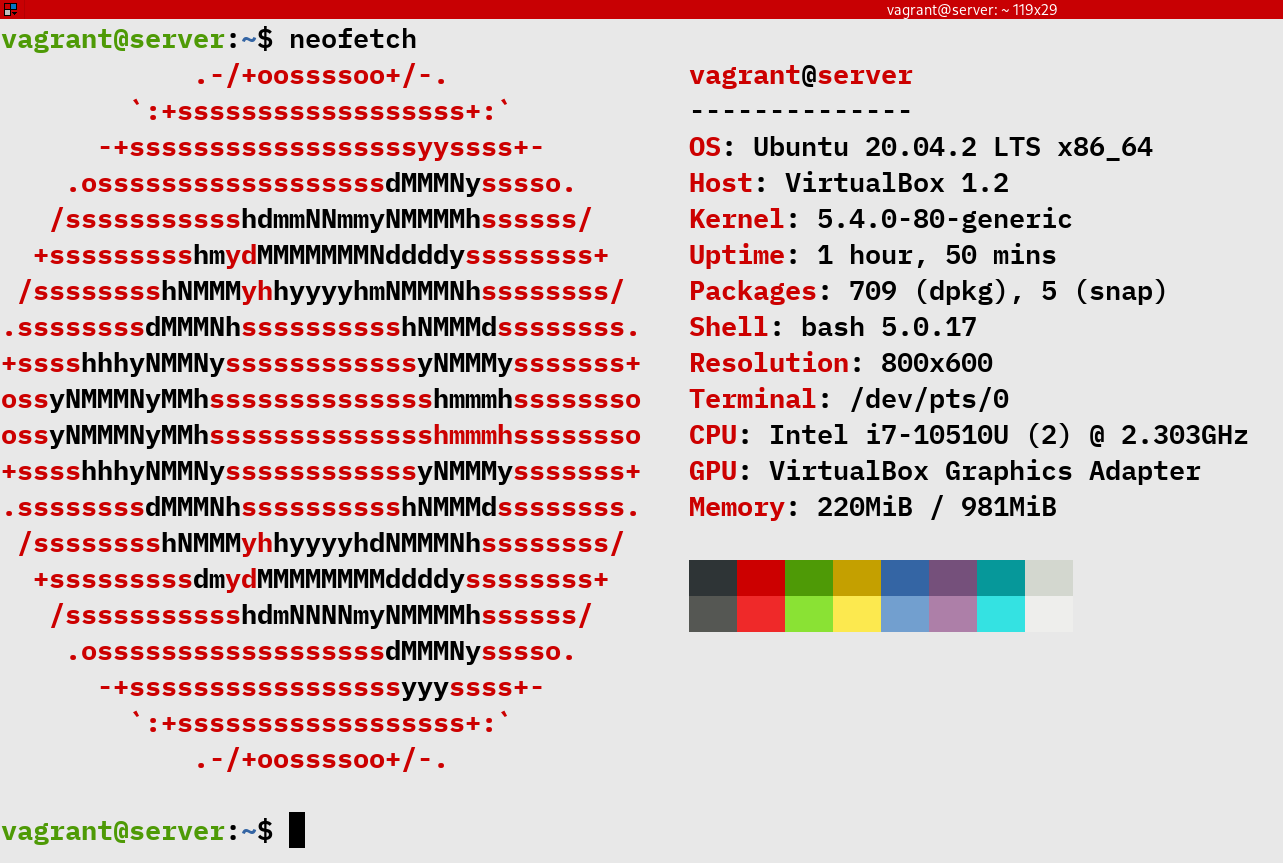
\includegraphics[width=.8\textwidth]{figures/_ubuntu.png}
    \label{fig:ubuntu}\caption{测试服务器 配置信息}
  \end{figure}
  
  